\documentclass[12pt,a4paper,final]{report}
\usepackage[utf8]{inputenc}
\usepackage[english]{babel}

% Package fo use of url
\usepackage{url}

% Packages for math symbols
\usepackage{amsmath}
\usepackage{amsfonts}
\usepackage{amssymb}
\usepackage[amssymb]{SIunits}

% Packages for images
\usepackage[final,pdftex]{graphicx}
\usepackage{float}

% Package for header
\usepackage{fancyhdr}
\setlength{\headheight}{15.2pt}
\renewcommand{\headrulewidth}{0pt}
\renewcommand{\footrulewidth}{0pt}

% Package for dividing sections
\usepackage{parskip}

\numberwithin{equation}{section}
\numberwithin{table}{section}
\numberwithin{figure}{section}

\renewcommand*\thesection{\arabic{section}} % fix to hide chapter number

\author{Hans-Kristian Bruvold\\Tom Eivind Glover\\Torkel Berli}
\title{Exercise 3 report}
\date{2013-03-15}

%\fancyhf{}

\renewcommand{\thispagestyle}[1]{} % do nothing


\begin{document}

\begin{titlepage} % TITLE ###################################

\pagestyle{fancy}
\chead{TDT4258 - Energy Efficient Computer Design}
\rhead{}
\cfoot{}
\begin{center}

\bigskip
\textbf{\LARGE REPORT}\\
\vspace{1.5cm}
\textnormal{\LARGE Exercise 3}\\
\vspace{1cm}
\textbf{\LARGE Linux driver and game}\\

\vspace{3cm}
by
\\
\vspace{0.5cm}
Hans-Kristian Bruvold\\
Tom Eivind Glover\\
Torkel Berli\\


\vspace{9cm}
Date: 2013-04-26

\end{center}

\end{titlepage} % END TITLE ###############################

\pagestyle{fancy}
\chead{}
\lhead{}


\section*{Abstract}
\label{sec:abstract} % a label to refer to

In this laboratory exercise we want to learn how to program kernel modules in C, learn how to program towards drivers on top of an operating system, and learn how to utilise linux for program development. The goal is to implement a game that runs on linux on the Atmel STK1000 Development Board, utilising the LCD screen, the DSP for sound, and its buttons and leds. We write drivers as kernel modules for linux for the buttons and leds. The finished game uses these buttons for controls, and the leds indicate some peripheral information. Existing drivers are used for communicating with LCD screen and DSP. A solid understanding of this development chain is critical for systems development where an operating system, and specifically linux, is involved.

\newpage

\tableofcontents

\newpage

\clearpage
\pagenumbering{arabic}

\cfoot{\thepage}

\section{Introduction}
\label{sec:introduction}
Microcontrollers often perform simple, specific tasks that can be programmed on “bare metal” . However, for larger and more complex applications, we need help from an operating system. An operating system provides an interface between our programs and the machine's hardware. The tasks it performs include reading and interpreting files and communicating with basic hardware like screen, hard drive, and other I/O elements. To communicate with these elements, the operating system uses drivers. Drivers are machine-native programs that run in the kernel (“in kernel space”) and communicate directly with the machine's hardware. In other words, without drivers, we would be unable to create programs that communicate with anything (or anyone). Learning how to write a kernel driver is important for low-level systems development.

An application that runs in user space can not, for good reasons, talk directly to a machine's hardware. Allowing this would make your machine free-for-all, letting anyone do whatever they wanted with it. Instead, when a user space application wants to communicate with the machine, it asks a kernel module (usually a driver) to perform the task on behalf the application. Through this, the kernel has control over what happens to the machine. The interface between user space and kernel space can be confusing and difficult to utilize, but it is important to learn how to take advantage of the utilities of existing drivers as well as your own self-written ones.

The I/O devices we will talk to in this exercise are button inputs, led outputs, screen output, and sound output, as well as reading files from disk. Button and led drivers will be written as part of the exercise. The drivers all work similarly. Using these drivers will be a game, also created in the exercise.

\newpage

\section{Methodology}
\label{sec:methodology}

\subsection{Atmel STK1000 development board}
\label{sec:stk1000}
\begin{figure}[H]
\centering
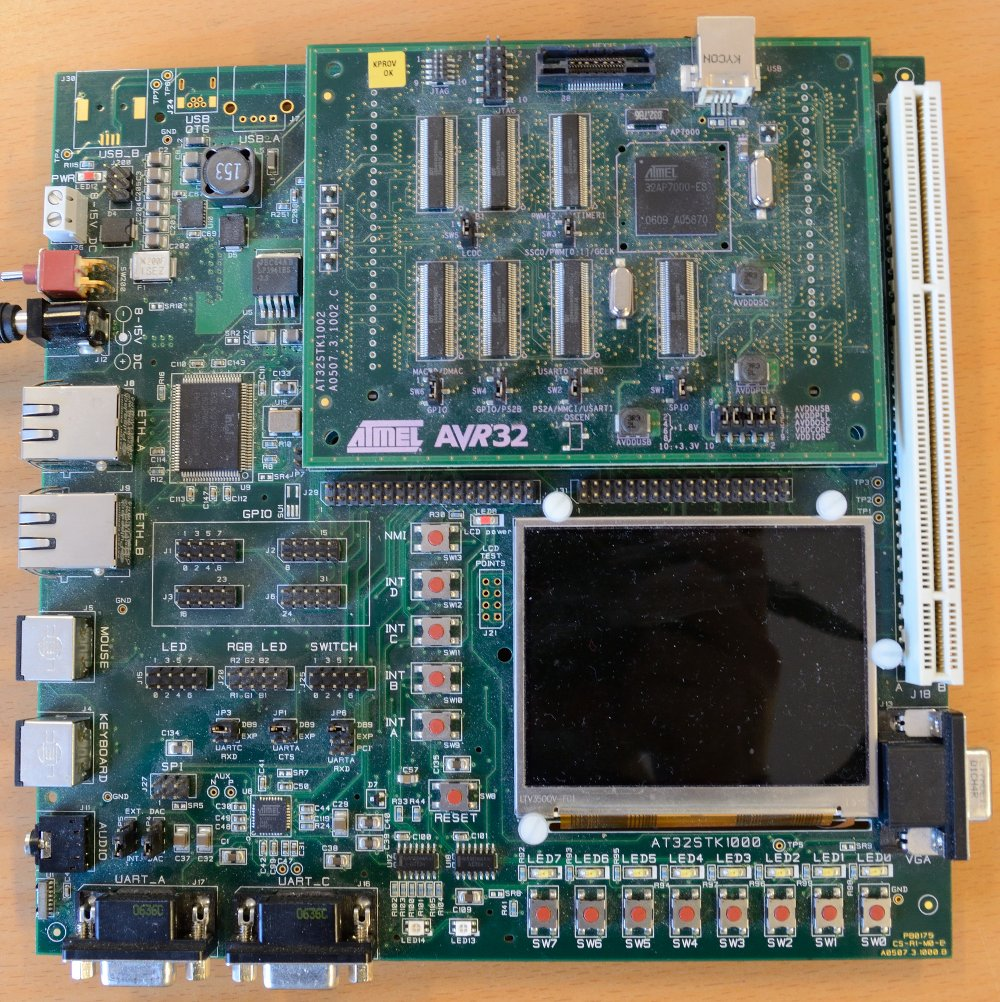
\includegraphics[scale=1.5]{stk1000photo}
\caption{Atmel STK1000 development board}
\label{fig:stk1000}
\end{figure}

In this exercise we will be using the display, buttons, LEDs and audio. These are features of the STK1000 development board. Since we will be using Linux we don’t have to get much into how these hardware features works, except for the buttons and LEDs, since we will write drivers for those. For data storage, the STK1000 has a SD card reader.

\subsection{GPIO - General Purpose Input Output}
\label{sec:gpio}

The LEDs and buttons can be controlled through the STK1000’s GPIO. The different pins on the GPIO can to some level be configured by using a set of ribbon cables. There are two ports from the microcontroller to the GPIO. Those are the PIOB and PIOC. Both has two 8-bit connector on the GPIO. The ribbon cables are connected to these connectors and to a IO device, like LEDs or buttons.

It is the PIO controller on the microcontroller that handles the buttons and LEDs. There is a set of memory addresses mapped to the PIO controller, these are used to configure the IO devices. Some of the relevant options are listed in table \ref{tab:pioregisters}

To use the LEDs there are two options that must be changed per pin in the PIO controller. Obviously, PER has to be set to enable the pin. And the second option is the OER, which tells the system that the pin is to be used as output, and not input as it is default.

In order to use the buttons there are also 2 options that must to be changed. The first is PER, to enable the pins. Then there is PUER, this will activate pull up resistors for the buttons.

\begin{table}[H]
\centering
\begin{tabular}{|l|l|}
\hline
Name & Register\\
\hline
PER & PIO Enable Register\\
PDR & PIO Disable Register\\
OER & Output Enable Register\\
PUER & Pull-Up Enable Register\\
SODR & Set Output Data Register\\
CODR & Clear Output Data Register\\
PDSR & Pin Data Status Register\\
\hline
\end{tabular}
\caption{Some of the control registers for the PIO Controller, for full list see page 262-263 in AT32AP7000 data sheet\cite{at32ap7000}}
\label{tab:pioregisters}
\end{table}


\subsection{Linux on the STK1000}
\label{sec:linuxstk1000}

Linux will be booted from the SD card. But in order to boot the SD card, the development board must be flashed with a bootloader. This can be done through a JTAG, Joint Test Action Group. The JTAG is used through Atmel’s programs for the STK1000.

When this is done, all that is left is to install Linux onto a SD card. Linux and its binaries has to be compiled towards the AVR32 instruction set. 

\subsection{Linux driver}
\label{sec:linuxdriver}

A Linux driver is a module that can be inserted into the kernel and act as a way for user applications to access hardware. There are two different types of drivers for Linux. One s character driver and the other is block driver. For controlling LEDs and buttons the character driver is the one which should be used. This is the most common type of driver, and it takes as input one byte a

a time. To clarify, the driver can take a greater input, but only one byte is interpretet at a time.

Since the driver might be used by several applications, the driver has to follow a standard for drivers. More specifically the driver needs a set of functions. The most essential functions are the functions for initialising and exiting. One is run when the driver is added to the Linux kernel. And the other is for when the driver is removed from the Linux kernel. Furthermore there are some structures, defined by struct in C,  that the driver needs. These are structure for file operations, like open, read, write, etc, and the second is information about the driver.

Each hardware device in Linux has a file in /dev directory. These files are used to access the devices. Every device file has its own major number and minor number. These numbers are used to link the file with a specific driver. So when something in written to a device file, the system looks for the driver associated with the major and minor number of the file, and then calls the write function from the driver. In the init function, the major and minor number must be registered. Other than registering major and minor number, the init function should also take care of kernel memory allocation if necessary and initialisation of the device the driver is for.

In the file operation structure, some functions must be defined in order for the driver to handle file operations on the device file. The basic ones are functions for open, close (release), read and write. The read, write, close and open functions are functions that are run when the device file is being read from, written to, closed and opened. The file structure is also registered in the init function.


\subsection{Display using /dev/fb0}
\label{sec:displayfb0}

The STK1000 LCD screen is called framebuffer (fb) and it controls the colors on each pixel on the screen. Through this, an application program can display whatever it wants on the screen, and it’s up to the application to display the wanted pattern. For instance, framebuffer cannot take text as input and print this to screen. It only sets int values for the color to each pixel to specified values.

\subsection{Sound using /dev/dsp}
\label{sec:sounddsp}

Using the /dev/dsp to play sound is an easy task. The sound driver only requires the sound data in order to play it. Sound can be played simply by writing raw sound data into /dev/dsp. The sound driver can also be configured by using linux/soundcard.h header. You are then able to change the bitrate or other settings concerning how you want the soundcard to handle your input.

\newpage

\section{Description}
\label{sec:description}

We started this exercise by making a Makefile for the driver. Then we made a simple driver which only printed out “Hello World”. This driver did not have any file operation structure or registration of major and minor number, but only the init and exit functions.

When we had the basic driver running, we knew that we had a setup capable of compiling Linux drivers for the AVR32 processor. From here on we could start developing the real drivers for LEDs and buttons.

\subsection{LED driver}
\label{sec:leddriver}

The LED driver has the init and exit functions. And for file operation it has a function for open, close (release), read and write. For controlling LED, the write function is the most important.

In the init function we used a function called alloc\_chrdev\_region(). This function lets the system choose a major and minor number for us. This way we avoid choosing a major number that is already used by another device. For accessing the device, we had to request access to a set of memory addresses. Since we wanted to run the LEDs through the PIOB port, we used the address for the PIOB and requested to use all the memory from PIOB to PIOC, which is 1024 addresses.  The third thing the init function did was to initialise the PIOB for the LEDs. And then lastly the init function registered the driver to the system.

The exit function only needed to release the address region for the PIOB and unregister the driver from the system. Because we chose to not allocate kernel memory, we didn’t have to release the memory space in the exit function.

The open, release and read functions of the driver are only empty functions. We did not need to do anything when the device file was opened or closed. And we figured it was not necessary to read from the LEDs.

The write function on the other hand, did update the LEDs. The function have two important parameters for accessing what was written to the driver. The first is the buffer (*buff), the buffer was a pointer to the data located in the user memory. The other is a count constant that told us how many bytes was written. Because of security reasons one should not write directly from the buffer and to the hardware. The correct way of using the buffer is to copy it from user memory to kernel memory. The function copy\_from\_user() does that in a safe way. So we used that function to copy what was written to the LED before the driver passed it on to the hardware. The function read, returns the number of bytes it read.

\subsection{Button driver}
\label{sec:buttondriver}

The button driver is in many way the same as the LED driver. It has support for the same file operations. The only difference in init (except for naming) is that it enables the pins for buttons. The exit function is pretty much the same.

The read function, however, is totally different. When the button device file is read, the read function is called. Here we have the parameters buffer (*buff) and count, which are important for us. The buffer parameter is a pointer to the user address that the data should be written to. We use the function copy\_to\_user() to copy the data read from the button hardware. The button data is read from the PDSR register in PIOB. Because we chose to have the buttons on PIOB as well as the LEDs, we have to do some logic to the data from the buttons. This is because button 0 to 7 is not addressed to 0x100 to 0x1FF. We solved this by checking every bits that are associated with the buttons. 


\subsection{LCD}
\label{sec:lcd}

For communicating with the LCD screen on the STK1000 we use a driver called framebuffer (fb). It gives us access to write to the pixels on the screen. To make this process easier, we use a tool called mmap(). Mmap() is a function that creates an array for us to write to, that routes directly to the input of the file given as one of the parameters. In this case, we get an array of all the pixels on the LCD screen. Or more specifically, an array of the three colors for each of the pixels for the screen.

Which brings us to an important point. The screen is made up of pixels. 320X240 of them. Each pixel consists of three bytes. The first one for blue, second one for green, and third byte is for red. These pixels have an unsigned value from 0 to 255, specifying the intensity of that color for that pixel. To set the desired color on a pixel, we have to write a value to each of these bytes. Therefore, our array for the input to the screen is 320*240*3 bytes = 230 400 bytes, or 225 kB.

\subsection{Sound}
\label{sec:sound}

To play sound we read from a sound file and wrote it to /dev/dsp. The process is pretty much straight forward. But the sound file must be completely raw. Which means that the only data in the file are the samples. To generate a raw sound file we used Audacity, and saved the file to 8 bit signed data without any header. 

\subsection{The game}
\label{sec:thegame}

The game implemented is a simple driving game in top-down view. The player controls a slick, red convertible with a confederate flag on the hood, and cruises along a dangerous road littered with obstacles. The player must avoid obstacles to save his ride. The more banged up his car becomes, the less chance he has at picking up chicks at his destination.

The controlled car is located at the bottom of the screen, and the game background scrolls down as he rides along. The background scrolling is a loop that shifts 1 pixel down 40 times a second (ie. Screen rate of 40Hz). A timer implemented in C returns to the executing function every 25 ms, and the executing function immediately paints the new picture. It then carries out the logic for what should be displayed on the next 25 ms tick.

The only things that change when the background scrolls are the stripes in the middle of the road and the stones of the sidewalk. To reduce bandwidth to the screen, only the pixels that change are actually written. This could be done because of the simple and predictable pattern change involved in scrolling down the road. This works similarly for the obstacles in the road. The controlled car is instead painted to the screen on each frame because of the more complicated picture and unpredictable direction of movement.

To control the car, the player has two buttons. One for steering right, and one for steering left. The LED lights below the LCD screen show how many obstacles the player has hit. All LED lights start out lit, and one is removed for every obstacle that is hit. When the player reaches the end of the map, the number of LED lights remaining is his score.


\newpage

\section{Testing and results}
\label{sec:testresults}

\subsection{Button and LED}
\label{sec:buttonandled}

To test the button and LED drivers we wrote 3 simple programs, ltest.c, btest.c and test.c. ltest.c would write 0x55 to the LED device. btest.c would read which buttons are pressed. test.c would start an infinite loop where it read the buttons and piped the button data into the LED device file.

We knew that we had the LED driver working when running the ltest program resulted the LEDs to turn on as expected. 0x55 means that every second LED would be turned on starting with the first LED. The LED driver also served as a tool for debugging as we used it to print kernel messages about relevant information.

btest would print a number representing what buttons are pressed. Pressing the first button and running the program would return 1, pressing the second button returns 2, the third 4, and so on. The button driver would also print kernel messages useful for debugging.

When we had both LED driver and button driver running, we tried the test program to check if both drivers worked at the same time. We knew it worked because when pressing a button, the LED next to the button would turn on.

\subsection{Display}
\label{sec:display}

Screen.c was the first test file we wrote to learn how to use existing linux kernel modules on the avr32. Actually, the first test we performed, after checking that the fb (framebuffer) driver was initialized, was the terminal command:

    \$ cat /boot/uImage \(> /dev/fb0

This command pipes the bytes in the kernel image on the development board (uImage) into the framebuffer input for the LCD screen. The driver certainly worked, the screen changed (into a mess). Screen.c was a test file to try to write to fb0 in C. Having already worked a lot on writing our own drivers, this was less of a hurdle. The essential commands were:

    fd = open("/dev/fb0", O\_RDWR \vline\ O\_CREAT \vline\ O\_TRUNC);

    screen=mmap(NULL, pixels*3, PROT\_READ \vline\ PROT\_WRITE, MAP\_SHARED, fd,0);

At first we just tried writing a flat color to the screen to see if we got any results. When this worked we could being drawing objects to locations on the screen, which involved more code and logic.

One issue we had in making this work was first not allowing reading, which prevented it from working properly. Afterwards, we weren't careful enough to match the permissions in the open() call with the permissions in mmap(), which also caused a problem. O\_CREAT and O\_TRUNC might not be necessary, but was thrown in because of their presence in a working example. After this test, we could go straight into mapping the pixels with mmap() (as explained in description), and work on drawing the board.

\subsection{Sound}
\label{sec:soundtest}

To test the sound we made a short sound file, test.raw, and a program, soundtest.c, that would read the file and write it to /dev/dsp. We had some issues with playing sound, so we tried to pipe /dev/urandom into /dev/dsp by running:

    \$ cat /dev/urandom \(> /dev/dsp

When we didn’t get any sound out of this command either, we knew that the problem was not in the soundtest.c, but somewhere else. It turned out to be that the sound driver was muted, we could unmute it through alsamixer. After unmuting, the soundtest.c worked as expected.

\newpage

\section{Discussion}
\label{sec:discussion}

\subsection{Drivers}
\label{sec:drivers}
The drivers worked well. But what could be changed with the drivers is that the LED driver could have a feature to be able to read from the LED device file to get what LEDs that are turned on. It is probably not necessary, but if more than one application is using the LEDs you would quickly end up in a conflict.

\subsection{LCD}
\label{sec:lcd2}
As mentioned in our tests, we took measures to limit the amount of bytes we wrote to the screen each tick. We did this to reduce flickering caused by overloading the screen. By later evaluating our game and by talking to other groups, we realized that the flickering was likely because of some pixels being written to more than once in each tick (with different colors). When the screen wrote two different and unrelated colors successively, the screen would seem to flicker. The work-around solution for us, by attempting to write to only the pixels that had changed, was a little tricky and also produced some non-perfect results when objects interacted with each other.

This is an area where we could have done more testing with writing to screen, to better understand the capabilities of our system. What we possibly could have done instead is keep a large array in memory that we could change like we wanted within each tick, and then at the end of the tick write that entire picture to screen. This would have caused us to overwrite the entire screen for each frame (requires a lot of bandwidth and memory), but it would ensure that we would not write to a pixel two times in the same frame (removing the flickering). 

\subsection{Improvements}
\label{sec:improvements}
We were unable to implement sound in the game. However the sound test program worked, so it was only the matter of time that limited us. We had plans about having a background music playing, and two different sound effects for events in the game (crashing into obstacle, and car horn).

The game is limited as of now. It does not have any obstacles, and because of this the score does not change. In further development of the game, sound, obstacles, and a score table would be the first features to be implemented. In making the game challenging, a natural feature would be to create harder and more obacles the further you got. Another fun feature would be multiplayer mode. Adding another car and two more buttons would let two players compete against eachother.

\newpage

\section{Conclusion}
\label{sec:conclusion}

This exercise included a great amount of skills and utilities, from hardware programming in the kernel module, to linux tools for development, to user interaction oriented C programming in the game. The work with the kernel and kernel modules was very enlightening for knowledge of how the operating system works, and for understanding the pipeline of calls that happen behind the scenes when application programs execute. When working with linux, we learned about utilities like ssh, scp, gcc, cat, grep, dmesg, insmod/rmmod/lsmod/chmod, to name a few. The final product, the game, leaves a lot to be desired. Firstly the game is not particularly well-structured with further modifications or development in mind. In other words, the game is not built on a defined game engine. Secondly, the game is relatively simple, and lacks typical things like high-score list and different levels, . It is generally short on finishing touches. Nonetheless, we are happy with making the chain of tools work properly, from hardware initializing to collision detection. The experience leaves us with a desire to further explore this kind of development.

\section{Glossary}
\label{sec:glossary}

\begin{table}[H]
\centering
\begin{tabular}{l l}
Kernel space & Part of virtual memory that is strictly reserved for running \\ & the kernel and its modules. Restricted.\\
User space & Part of virtual memory for applications running on top of\\ & the operating system. Each application has its own separate\\ & space here.\\
Kernel module & A program in kernel space that serves as an extension for the\\ & operating system.\\
DSP & Digital Signal Processor. We use this for outputting sound.\\
AVR32 & The instruction set and architecture of the processor being used.\\
STK1000 & The development board being used.\\
\end{tabular}
\label{tab:glossary}
\end{table}

\bibliographystyle{plain}
\bibliography{bibliography}

\end{document}
